\documentclass{article}

\usepackage{polski}
\usepackage[utf8]{inputenc}
\usepackage{indentfirst}
\usepackage{color}
\usepackage{graphicx}

\newcommand{\TODO}[1]{\textcolor{blue}{TODO: #1}}
\newcommand{\ang}[1]{ang.~{\itshape #1}}

\begin{document}

\title{Metody odkrywania wiedzy \\%
{\large Klasyfikacja -- dokumentacja końcowa} }

\author{Jakub Cichanowicz \and Artur Sawicki}

\maketitle

\section{Analiza i przygotowanie danych}
W zbiorze danych mamy 12 zmiennych. Część z nich ma braki, które należy uzupełnić, gdyż nie wszystkie algorytmy radzą sobie z brakami danych.

\subsection{Klasa pasażerska}

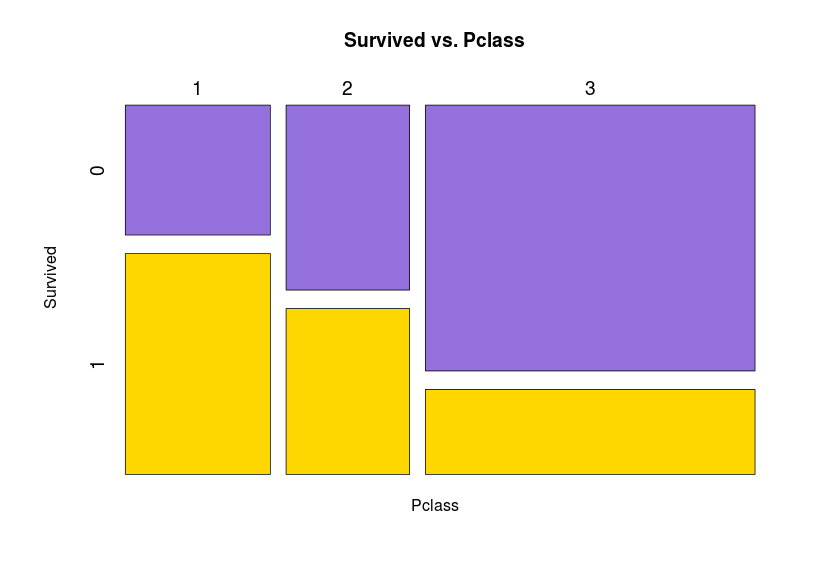
\includegraphics[scale=0.40]{images/survived-vs-pclass.png}

\subsection{Płeć}

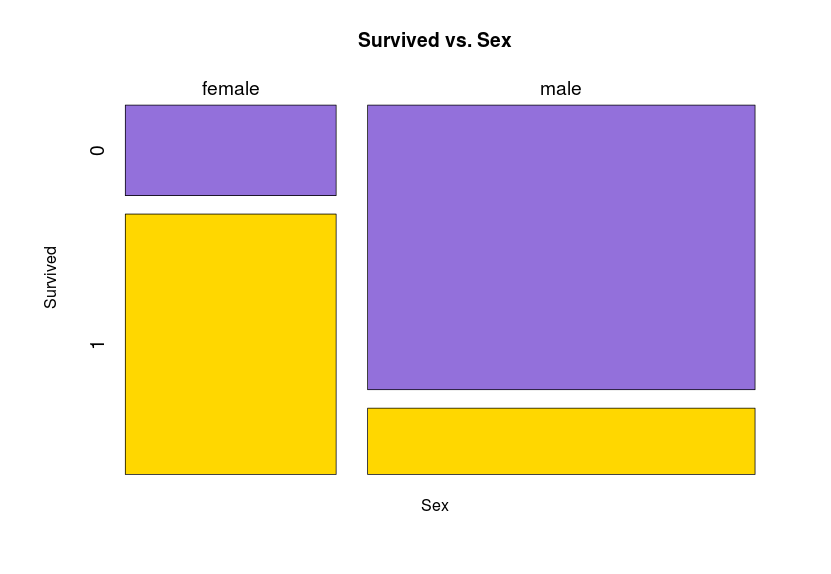
\includegraphics[scale=0.40]{images/survived-vs-sex.png}

\subsection{Wiek}

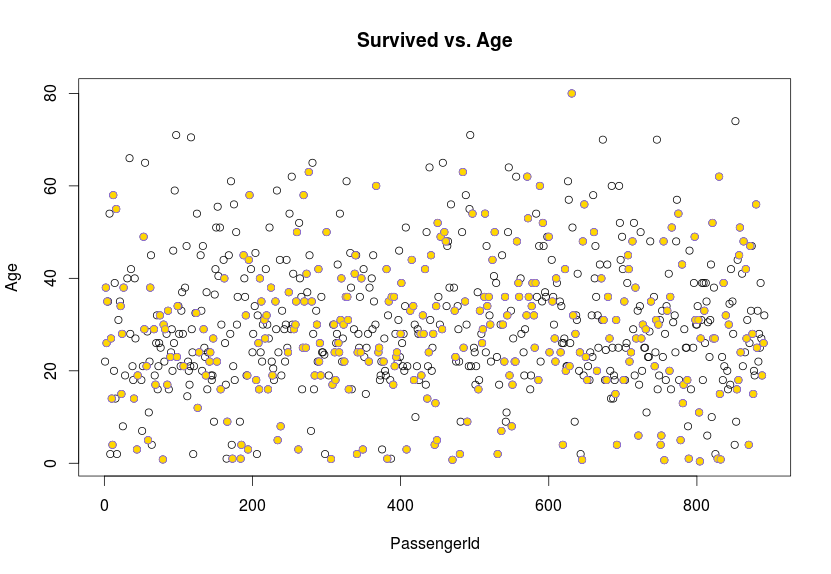
\includegraphics[scale=0.40]{images/survived-vs-age.png}

\subsection{Liczba rodzeństwa/małżonków na pokładzie}

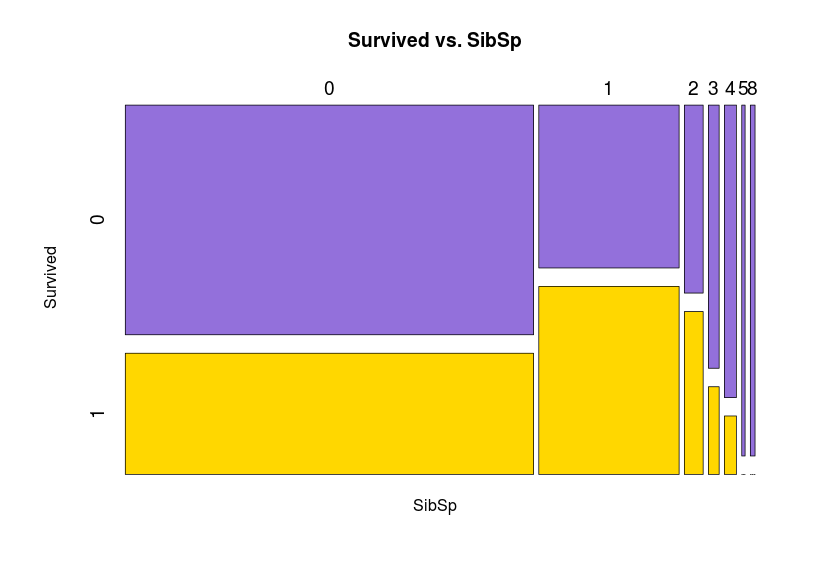
\includegraphics[scale=0.40]{images/survived-vs-sibsp.png}

\subsection{Liczba dzieci/rodziców na pokładzie}

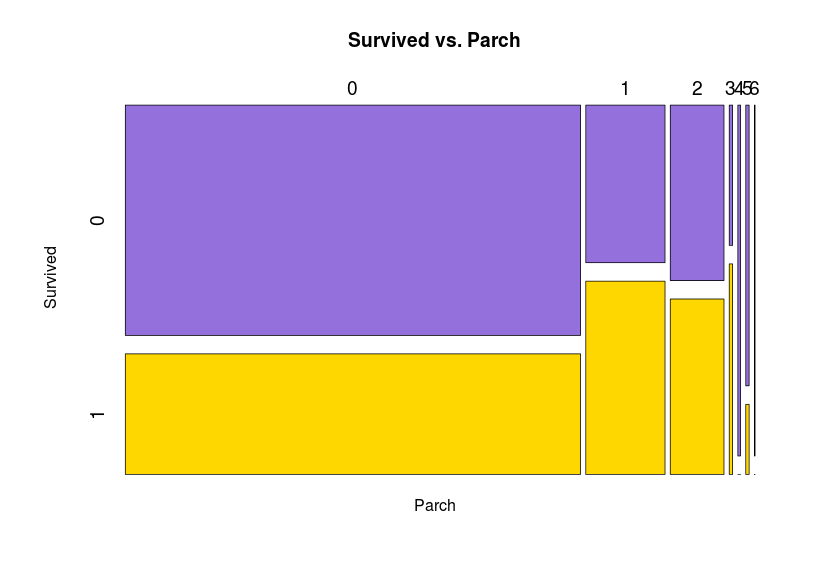
\includegraphics[scale=0.40]{images/survived-vs-parch.png}

\subsection{Opłata}

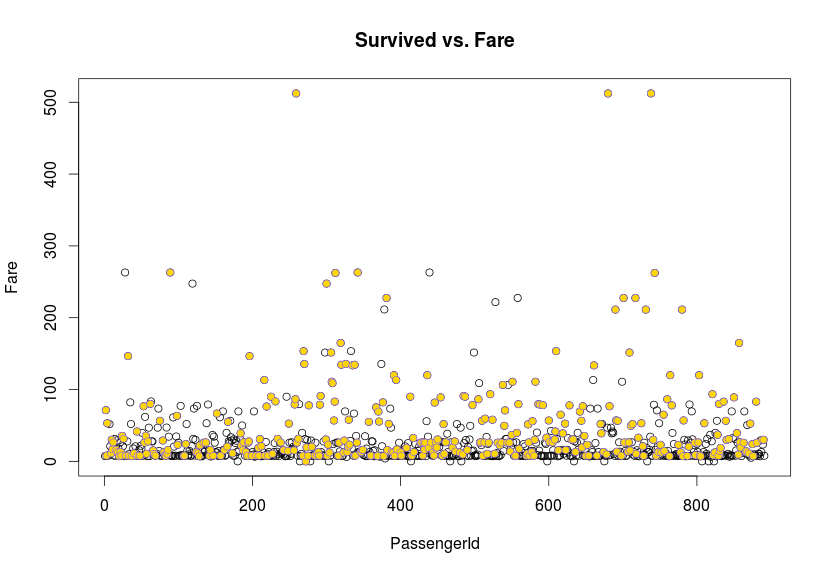
\includegraphics[scale=0.40]{images/survived-vs-fare.png}
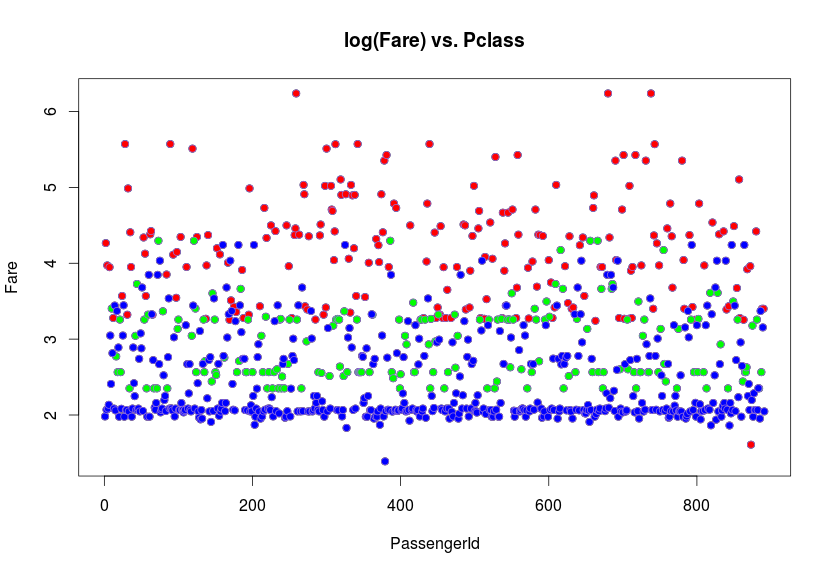
\includegraphics[scale=0.40]{images/logfare-vs-pclass.png}

\subsection{Miejsce wejścia na pokład }

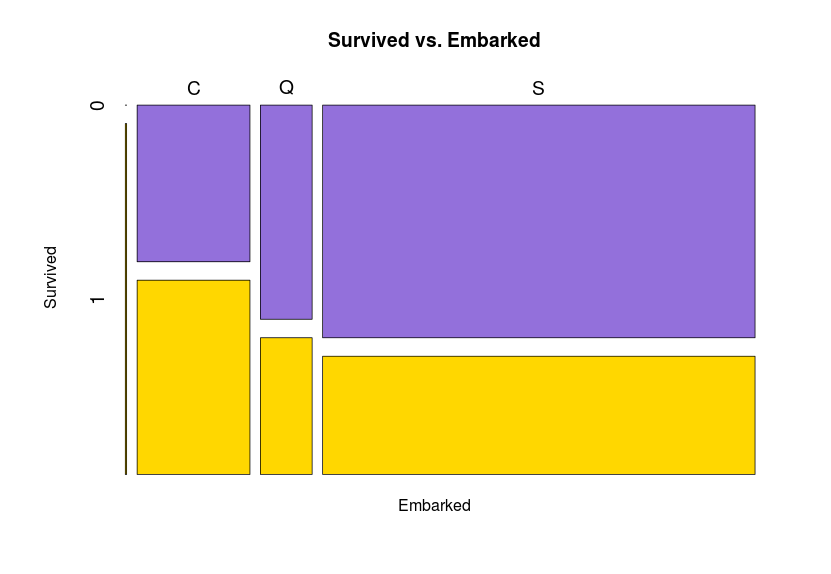
\includegraphics[scale=0.40]{images/survived-vs-embarked.png}

\section{Selekcja atrybutów}
\section{Kalibracja}
\section{Tworzenie modeli}
\section{Ocena jakości modeli}
\section{Podsumowanie}

\end{document}
